%% This file is a portion of the source for Revised Edition 1.1 of
%% Operating Systems and Middleware: Supporting Controlled
%% Interaction, Copyright 2011 by Max Hailperin.  This work is
%% licensed under the Creative Commons Attribution-ShareAlike 3.0
%% Unported License. To view a copy of this license, visit
%% http://creativecommons.org/licenses/by-sa/3.0/ or send a letter to
%% Creative Commons, 171 Second Street, Suite 300, San Francisco,
%% California, 94105, USA.
\chapter{Introduction}\label{intro-chapter}

\section{Chapter Overview}

This book covers a lot of ground.  In it, I will explain to you the basic
principles that underlie a broad range of systems and also give you
concrete examples of how those principles play out in several specific
systems.  You will see not only some of the internal workings of
low-level infrastructure, but also how to build
higher-level applications on top of that infrastructure to make use of
its services.  Moreover, this book will draw on material you may have encountered in
other branches of computer science and engineering and engage you in
activities ranging from mathematical proofs to the experimental
measurement of real-world performance and the consideration of how
systems are used and abused in social context.

Because the book as a whole covers so much ground, this chapter is
designed to give you a quick view of the whole terrain, so that you
know what you are getting into.  This is especially important because
several of the topics I cover are interrelated, so that even though I
carefully designed the order of presentation, I am still going to confront
you with occasional forward references. You will find, however, that this introductory chapter
gives you a sufficient overview of all the topics so that you won't
be mystified when a chapter on one makes some reference to another.

In Section~\ref{what-is-os-section}, I will explain what an operating
system is, and in Section~\ref{what-is-middleware-section}, I will do
the same for middleware.  After these two sections, you will know
what general topic you are studying.
Section~\ref{book-objectives-section} gives you some reasons
for studying that topic, by explaining several roles that I hope this
book will serve for you.

After the very broad overview provided by these initial sections, the
remaining sections of this chapter are somewhat more focused.  Each
corresponds to one or more of the later chapters and explains one
important category of service provided by operating systems and
middleware.
Section~\ref{concurrency-section} explains how a single computer can
run several computations concurrently, a topic addressed in more depth
by Chapters \ref{threads-chapter} and \ref{scheduling-chapter}.
Section~\ref{controlled-interaction-section} explains how interactions
between those concurrent computations can be kept under control, the
topic of Chapters \ref{synchronization-chapter} through
\ref{processes-chapter}.  Sections \ref{persistence-section} and
\ref{networking-section} extend the range of interacting computations
across time and space, respectively, through mechanisms such as file
systems and networking.  They preview
Chapter~\ref{persistence-chapter} and Chapters
\ref{networking-chapter} and \ref{distmid-chapter}.  Finally,
Section~\ref{intro-security-section} introduces the topic of security,
a topic I revisit at the end of each chapter and then focus on in
Chapter~\ref{security-chapter}.

\section{What Is an Operating System?}\label{what-is-os-section}

An \vocab{operating system} is software that uses the hardware
resources of a computer system to provide support for the execution of
other software.  Specifically, an operating system provides the
following services:
\begin{itemize}
\item
The operating system allows multiple computations to take place
concurrently on a single computer system.  It divides the hardware's
time between the computations and handles the shifts of focus between
the computations, keeping track of where each one leaves off so that
it can later correctly resume.
\item
The operating system controls the interactions between the concurrent
computations.  It can enforce rules, such as forbidding computations
from modifying data structures while other computations are accessing
those structures.  It can also provide isolated areas of memory for
private use by the different computations.
\item
The operating system can provide support for controlled
interaction of computations even when they do not run concurrently.
In particular, general-purpose operating systems provide file systems,
which allow computations to read data from files written by earlier
computations.  This feature is optional because an embedded system,
such as the computer controlling a washing machine, might in some
cases run an operating system, but not provide a file system or other
long-term storage.
\item
The operating system can provide support for
controlled interaction of computations spread among different computer
systems by using networking. This is another standard feature of
general-purpose operating systems.
\end{itemize}
These services are illustrated in Figure~\ref{scan-1-1}.
\begin{figure}
\centerline{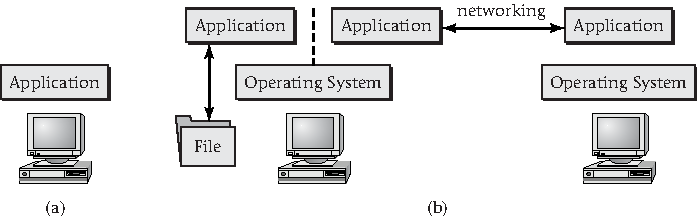
\includegraphics{hail_f0101}}
\caption{Without an operating system, a computer can directly execute
  a single program, as shown in part (a).  Part (b) shows that with an operating system,
  the computer can support concurrent computations, control the
  interactions between them (suggested by the dashed line), and allow
  communication across time and space by way of files and networking.}
\label{scan-1-1}
\end{figure}

If you have programmed only general-purpose computers, such as PCs,
workstations, and servers, you have probably never encountered a
computer system that was not running an operating system or that did
not allow multiple computations to be ongoing.  For example, when you
boot up your own computer, chances are it runs Linux, Microsoft
Windows, or Mac OS~X and that you can run multiple application
programs in individual windows on the display screen.  These three
operating systems will serve as my primary examples throughout the
book.

To illustrate that a computer can run a single program without an
operating system, consider embedded systems.  A typical
embedded system might have neither keyboard nor display screen.
Instead, it might have temperature and pressure sensors and an output
that controls the fuel injectors of your car.  Alternatively, it might have
a primitive keyboard and display, as on a microwave oven, but still
be dedicated to running a single program.

Some of the most sophisticated embedded systems run multiple
cooperating programs and use operating systems.  However, more
mundane embedded systems take a simpler form.  A single program is
directly executed by the embedded processor.  That program contains
instructions to read from input sensors, carry out appropriate
computations, and write to the output devices.  This sort of embedded
system illustrates what is possible without an operating system.  It
will also serve as a point of reference as I contrast my definition of an
operating system with an alternative definition.

One popular alternative definition of an operating system is that it
provides application programmers with an abstract view of the
underlying hardware resources, taking care of the low-level details so
that the applications can be programmed more simply.  For example, the
programmer can write a simple statement to output a string without
concern for the details of making each character appear on the display
screen.

I would counter by remarking that abstraction can be provided without
an operating system, by linking application programs with separately
written libraries of supporting procedures.  For example, a program
could output a string using the standard mechanism of a programming
language, such as C$++$ or Java.  The application programmer would not
need to know anything about hardware.  However, rather than running on an
operating system, the program could be linked together with a library
that performed the output by appropriately manipulating a microwave
oven's display panel.  Once running on the oven's embedded processor,
the library and the application code would be a single program,
nothing more than a sequence of instructions to directly execute.
However, from the application programmer's standpoint, the low-level
details would have been successfully hidden.

To summarize this argument, a library of input/output routines is not
the same as an operating system, because it satisfies only the first
part of my definition.  It does use underlying hardware to support the
execution of other software.  However, it does not provide support for
controlled interaction between computations.  In fairness to the
alternative viewpoint, it is the more historically grounded one.
Originally, a piece of software could be called an operating system
without supporting controlled interaction.  However, the language has
evolved such that my definition more closely reflects current usage.

I should also address one other alternative view of operating systems,
because it is likely to be the view you have formed from your own
experience using general-purpose computers.  You are likely to think
of an operating system as the software with which you interact in order to
carry out tasks such as running application programs.  Depending on
the user interface to which you are accustomed, you might think the
operating system is what allows you to click program icons to run
them, or you might think the operating system is what interprets
commands you type.

There is an element of truth to this perception.  The operating system
does provide the service of executing a selected application program.
However, the operating system provides this service not to human users
clicking icons or typing commands, but to other programs already
running on the computer, including the one that handles icon clicks or
command entries.  The operating system allows one program that is
running to start another program running.  This is just one of the
many services the operating system provides to running programs.
Another example service is
writing output into a file.  The sum total of features the
operating system makes available for application programmers to use in
their programs is called the \vocab{Application Programming Interface}
(\vocab{API}).  One element of the API is the ability to run other programs.

The reason why you can click a program icon or type in a command to
run a program is that general-purpose operating systems come bundled
with a user-interface program, which uses the operating system API to
run other programs in response to mouse or keyboard input.  At a
marketing level, this user-interface program may be treated as a part of
the operating system; it may not be given a prominent name of its own
and may not be available for separate purchase.

For example, Microsoft Windows comes with a user interface known as
Explorer, which provides features such as the Start menu and the
ability to click icons.  (This program is distinct from the
similarly named web browser, Internet Explorer.)  However, even if you
are an experienced Windows user, you may never have heard of Explorer;
Microsoft has chosen to give it a very low profile, treating it as an
integral part of the Microsoft Windows environment.  At a technical
level, however, it is distinct from the operating system proper.  In
order to make the distinction explicit, the true operating system is
often called the \vocab{kernel}.  The kernel is the fundamental
portion of Microsoft Windows that provides an API supporting
computations with controlled interactions.

A similar distinction between the kernel and the user interface
applies to Linux.  The Linux kernel provides the basic operating
system services through an API, whereas \vocabs{shell} are the
programs (such as bash and tcsh) that interpret typed commands, and
\vocabs{desktop environment} are the programs, such as KDE (K Desktop Environment) and GNOME,
that handle graphical interaction.

In this book, I will explain the workings of operating system
kernels, the true operating systems themselves, as opposed to the
user-interface programs.  One reason is because user-interface programs
are not constructed in any fundamentally different way than normal
application programs.  The other reason is because an operating system
need not have this sort of user interface at all.  Consider again the
case of an embedded system that controls automotive fuel
injection.  If the system is sufficiently sophisticated, it may
include an operating system.  The main control program may run other,
more specialized programs.  However, there is no ability for the user
to start an arbitrary program running through a shell or desktop
environment.  In this book, I will draw my examples from
general-purpose systems with which you might be familiar, but will emphasize
the principles that could apply in other contexts as well.

\section{What is Middleware?}\label{what-is-middleware-section}

Now that you know what an operating system is, I can turn to the other
category of software covered by this book: \vocab{middleware}.  Middleware is software occupying a middle
position between application programs and operating systems, as I will
explain in this section.

Operating
systems and middleware have much in common.  Both are software used to
support other software, such as the application programs you run.
Both provide a similar range of services centered around controlled
interaction.  Like an operating system, middleware may enforce rules
designed to keep the computations from interfering with one another.
An example is the rule that only one computation may modify a shared data structure
at a time.  Like an operating system, middleware may bring
computations at different times into contact through persistent
storage and may support interaction between computations on different
computers by providing network communication services.

Operating systems and middleware are not the same, however.  They rely upon
different underlying providers of lower-level services.  An
operating system provides the services in its API by making use of the
features supported by the hardware.  For example, it might provide API
services of reading and writing named, variable-length files by making
use of a disk drive's ability to read and write numbered, fixed-length
blocks of data.  Middleware, on the other hand, provides the services
in its API by making use of the features supported by an underlying
operating system.  For example, the middleware might provide API
services for updating relational database tables by making use of an
operating system's ability to read and write files that contain the database.

This layering of middleware on top of an operating system, as illustrated
in Figure~\ref{scan-1-2}, explains the
name; middleware is in the middle of the vertical stack, between the
application programs and the operating system.
\begin{figure}
\centerline{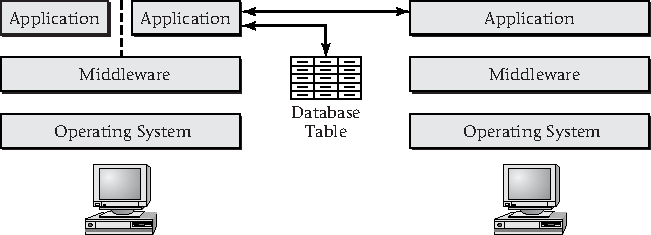
\includegraphics{hail_f0102}}
\caption{Middleware uses services from an operating system and in turn
provides services to application programs to support controlled interaction.}
\label{scan-1-2}
\end{figure}
Viewed horizontally rather than vertically, middleware is also in the
middle of interactions between different application programs
(possibly even running on different computer systems), because it
provides mechanisms to support controlled interaction through
coordination, persistent storage, naming, and communication.

I already mentioned relational database systems as one example of
middleware.  Such systems provide a more sophisticated form of persistent storage
than the files supported by most operating systems.  I use Oracle as
my primary source of examples regarding relational database systems.
Other middleware I will use for examples in the book includes the
Java~2 Platform, Enterprise Edition (J2EE) and IBM's WebSphere MQ.  These
systems provide support for keeping computations largely isolated from
undesirable interactions, while allowing them to communicate with one
another even if running on different computers.

The marketing definition of middleware doesn't always correspond
exactly with my technical definition.  In particular, some middleware
is of such fundamental importance that it is distributed as part of
the operating system bundle, rather than as a separate middleware
product.  As an example, general-purpose operating systems all come
equipped with some mechanism for translating Internet hostnames, such as
\textit{www.gustavus.edu}, into numerical addresses.  These mechanisms are
typically outside the operating system kernel, but provide a general
supporting service to application programs.  Therefore, by my
definition, they are middleware, even if not normally labeled as such.

\section{Objectives for the Book}\label{book-objectives-section}

If you work your way through this book, you will gain both knowledge
and skills.  Notice that I did not say anything about {\em reading}
the book, but rather about {\em working your way through} the book.
Each chapter in this book concludes with exercises, programming
projects, exploration projects, and some bibliographic or historical
notes.  To achieve the objectives of the book, you need to work
exercises, carry out projects, and occasionally venture down one of
the side trails pointed out by the end-of-chapter notes.  Some of the
exploration projects will specifically direct you to do research in
outside sources, such as on the Internet or in a library.  Others will
call upon you to do experimental work, such as measuring the
performance consequences of a particular design choice. If you are
going to invest that kind of time and effort, you deserve some idea of
what you stand to gain from it.  Therefore, I will explain in the
following paragraphs how you
will be more knowledgeable and skilled after finishing the book.

First, you will gain a general knowledge of how contemporary operating
systems and middleware work and some idea why they work that way.
That knowledge may be interesting in its own right, but it also has
practical applications.  Recall that these systems provide supporting
APIs for application programmers to use.  Therefore, one payoff will
be that if you program applications, you will be positioned to make
more effective use of the supporting APIs.  This is true even though
you won't be an expert at any particular API; instead, you'll see the
big picture of what services those APIs provide.

Another payoff will be if you are in a role where you need to alter
the configuration of an operating system or middleware product in order to
tune its performance or make it best serve a particular context.
Again, this one book alone won't give you all the specific knowledge
you need about any particular system, but it will give you the general
background to make sense out of more specialized references.

Perhaps the most significant payoff for learning the details
of today's systems in the context of the reasons behind their designs
is that you will be in a better position to learn tomorrow's systems.
You will be able to see in what ways they are different and in what
ways they are fundamentally still the same.  You will be able to put
new features into context, often as a new solution to an old problem,
or even just as a variant on an existing solution.  If you really get
excited by what you learn from this book, you could even use your
knowledge as the foundation for more advanced study and become one of
the people who develops tomorrow's systems.

Second, in addition to knowledge about systems, you will learn some
skills that are applicable even outside the context of operating
systems and middleware.  Some of the most important skills come from the
exploration projects.  For example, if you take those projects
seriously, you'll practice not only conducting experiments, but also
writing reports describing the experiments and their results.  That
will serve you well in many contexts.

I have also
provided you with some opportunities to develop proficiency in using the
professional literature, such as
documentation and the papers published in conference proceedings.
Those sources go into more depth than this book can, and they will
always be more up-to-date.

From the programming projects, you'll gain some skill at writing
programs that have several interacting components operating
concurrently with one another and that keep their interactions under
control.  You'll also develop some skill at writing programs that
interact over the Internet.  In neither case will you become a master
programmer.  However, in both cases, you will be laying a foundation of
skills that are relevant to a range of development projects and
environments.

Another example of a skill you can acquire is the ability to look at
the security ramifications of design decisions.  I have
a security section in each chapter, rather than a security
chapter only at the end of the book, because I want you to develop the
habit of asking, ``What are the security issues here?''  That question
is relevant even outside the realm of operating systems and
middleware.

As I hope you can see, studying operating systems and middleware can
provide a wide range of benefits, particularly if you engage yourself
in it as an active participant, rather than as a spectator.  With that
for motivation, I will now take you on another tour of the services
operating systems and middleware provide.  This tour is more detailed than
Sections \ref{what-is-os-section} and
\ref{what-is-middleware-section}, but not as detailed as Chapters
\ref{threads-chapter} through \ref{security-chapter}.

\section{Multiple Computations on One Computer}\label{concurrency-section}

The single most fundamental service an operating system provides is to
allow multiple computations to be going on at the same time, rather
than forcing each to wait until the previous one has run to
completion.  This allows desktop computers to juggle multiple tasks
for the busy humans seated in front of their screens, and it allows
server computers to be responsive to requests originating from many
different client computers on the Internet.  Beyond these
responsiveness concerns, concurrent computations can also make more
efficient use of a computer's resources.  For example, while one
computation is stalled waiting for input to arrive, another
computation can be making productive use of the processor.

A variety of words can be  used to refer to the computations underway
on a computer; they may be called threads, processes, tasks, or jobs.
In this book, I will use both the word ``thread'' and the word
``process,'' and it is important that I explain now the difference
between them.

A \vocab{thread} is the fundamental unit of concurrency.  Any one sequence of
programmed actions is a thread.  Executing a program might create
multiple threads, if the program calls for several independent
sequences of actions run concurrently with one another.  Even if each
execution of a program creates only a single thread, which is the more
normal case, a typical system will be running several threads: one for
each ongoing program execution, as well as some that are internal
parts of the operating system itself.

When you start a program running, you are always creating one or more
threads.  However, you are also creating a \vocab{process}.  The process is a
container that holds the thread or threads that you started running and
protects them from unwanted interactions with other unrelated
threads running on the same computer.  For example, a thread running
in one process cannot accidentally overwrite memory in use by a
different process.

Because human users normally start a new process running every time
they want to make a new computation happen, it is tempting to think of
processes as the unit of concurrent execution.  This temptation is
amplified by the fact that older operating systems required each
process to have exactly one thread, so that the two kinds of object
were in one-to-one correspondence, and it was not important to
distinguish them.  However, in this book, I will consistently make
the distinction.  When I am referring to the ability to set an
independent sequence of programmed actions in motion, I will write
about creating threads.  Only when I am referring to the ability to
protect threads will I write about creating processes.

In order to support threads, operating system APIs include features
such as the ability to create a new thread and to kill off an
existing thread.  Inside the operating system, there must be some
mechanism for switching the computer's attention between the various
threads.  When the operating system suspends execution of one thread
in order to give another thread a chance to make progress, the
operating system must store enough information about the first thread
to be able to successfully resume its execution later.
Chapter~\ref{threads-chapter} addresses these issues.

Some threads may not be runnable at any particular time, because they
are waiting for some event, such as the arrival of input.  However, in
general, an operating system will be confronted with multiple runnable
threads and will have to choose which ones to run at each
moment.  This problem of scheduling threads' execution has many
solutions, which are surveyed in Chapter~\ref{scheduling-chapter}.
The scheduling problem is interesting, and has generated
so many solutions, because it involves the balancing of system
users' competing interests and values.  No individual scheduling approach
will make everyone happy all the time.  My focus is on explaining how
the different scheduling approaches fit different contexts of system
usage and achieve differing goals.  In addition I explain how APIs allow
programmers to exert control over scheduling, for example, by
indicating that some threads should have higher priority than others.

\section{Controlling the Interactions Between
  Computations}\label{controlled-interaction-section}

Running multiple threads at once becomes more interesting if the
threads need to interact, rather than execute completely
independently of one another.  For example, one thread might be
producing data that another thread consumes.  If one thread is writing
data into memory and another is reading the data out, you don't want
the reader to get ahead of the writer and start reading from locations
that have yet to be written.  This illustrates one broad family of
control for interaction: control over the relative timing of the
threads' execution.  Here, a reading step must take place after the
corresponding writing step.  The general name for control over
threads' timing is \vocab{synchronization}.

Chapter~\ref{synchronization-chapter} explains several common
synchronization patterns, including keeping a consumer from
outstripping the corresponding producer.  It also explains the
mechanisms that are commonly used to provide synchronization, some of
which are supported directly by operating systems, while others
require some modest amount of middleware, such as the Java runtime
environment.

That same chapter also explains a particularly important difficulty
that can arise from the use of synchronization.  Synchronization can
force one thread to wait for another.  What if the second thread
happens to be waiting for the first?  This sort of cyclic waiting is
known as a \vocab{deadlock}.  My discussion of ways to cope with deadlock
also introduces some significant
middleware, because database systems provide an interesting example of
deadlock handling.

In Chapter~\ref{transactions-chapter}, I expand on the themes of
synchronization and middleware by explaining transactions, which are
commonly supported by middleware.  A \vocab{transaction} is a unit of
computational work for which no intermediate state from the middle of
the computation is ever visible.  Concurrent transactions are isolated
from seeing each other's intermediate storage.  Additionally, if a
transaction should fail, the storage will be left as it was before the
transaction started.
Even if the computer system should catastrophically crash in the middle of a transaction's execution, the storage after rebooting will not reflect the partial transaction.
This prevents results of a half-completed
transaction from becoming visible.  Transactions are incredibly useful
in designing reliable information systems and have widespread
commercial deployment.  They also provide a good example of how
mathematical reasoning can be used to help design practical systems;
this will be the chapter where I most prominently expect you to
understand a proof.

Even threads that have no reason to interact may accidentally
interact, if they are running on the same computer and sharing the same
memory.  For example, one thread might accidentally write into memory being used by
the other.  This is one of several reasons why operating systems
provide \foldvocab{virtual}{memory}, the topic of
Chapter~\ref{vm-chapter}.  Virtual memory refers to the technique of
modifying addresses on their way from the processor to the memory, so
that the addresses actually used for storing values in memory may be
different from those appearing in the processor's load and store
instructions.  This is a general mechanism provided through a
combination of hardware and operating system software.  I explain
several different goals this mechanism can serve, but the most
simple is isolating threads in one process from those in another by
directing their memory accesses to different regions of memory.

Having broached the topic of providing processes with isolated virtual
memory, I devote
Chapter~\ref{processes-chapter} to processes.  This chapter explains an API for
creating processes.  However, I also focus on protection
mechanisms, not only by building on Chapter~\ref{vm-chapter}'s introduction
of virtual memory, but also by explaining other forms of protection
that are
used to protect processes from one another and to protect the
operating system itself from the processes.  Some of these protection
mechanisms can be used to protect not just the storage of values in memory,
but also longer-term data storage, such as files, and even network
communication channels.  Therefore, Chapter~\ref{processes-chapter}
lays some groundwork for the later treatment of these topics.

Chapter~\ref{processes-chapter} also provides me an opportunity to
clarify one point about threads left open by
Chapter~\ref{threads-chapter}.  By showing how operating systems
provide a protective boundary between themselves and the running
application processes, I can explain where threads fall relative to
this boundary.  In particular, there are threads that are contained
entirely within the operating system kernel, others that are contained entirely
within an application process, and yet others that cross the boundary,
providing support from within the kernel for concurrent activities
within the application process.  Although it might seem natural to
discuss these categories of threads in Chapter~\ref{threads-chapter},
the chapter on threads, I really need to wait for
Chapter~\ref{processes-chapter} in order to make any more sense out of
the distinctions than I've managed in this introductory paragraph.

When two computations run concurrently on a single computer, the hard
part of supporting controlled interaction is to keep the interaction
under control.  For example, in my earlier example of a
pair of threads, one produces some data and the other consumes it.
In such a situation, there is no great mystery to how the data can flow from one to the
other, because both are using the same computer's memory.  The hard
part is regulating the use of that shared memory.  This stands in
contrast to the interactions across time and space, which I will address in Sections
\ref{persistence-section} and \ref{networking-section}.  If the producer and consumer run
at different times, or on different computers, the operating system
and middleware will need to take pains to convey the data from one to
the other.

\section{Supporting Interaction Across Time}\label{persistence-section}

General purpose operating systems all support some mechanism for
computations to leave results in long-term storage, from which they can be
retrieved by later computations.  Because this storage persists even
when the system is shut down and started back up, it is known as
\foldvocab{persistent}{storage}.  Normally, operating systems provide
persistent storage in the form of named files, which are organized into a
hierarchy of directories or folders.  Other forms of persistent
storage, such as relational database tables and application-defined
persistent objects, are generally supported by middleware.  In
Chapter~\ref{persistence-chapter}, I focus on file systems, though I
also explain some of the connections with middleware.  For example, I
compare the storage of file directories with that of database
indexes.  This comparison is particularly important as these areas are
converging.  Already the underlying mechanisms are very similar, and
file systems are starting to support indexing services like
those provided by database systems.

There are two general categories of file APIs, both of which I cover
in Chapter~\ref{persistence-chapter}.  The files can be made a part of
the process's virtual memory space, accessible with normal load and
store instructions, or they can be treated separately, as external
entities to read and write with explicit operations.

Either kind of file API provides a relatively simple interface to some
quite significant mechanisms hidden within the operating system.
Chapter~\ref{persistence-chapter} also provides a survey of some of
these mechanisms.

As an example of a simple interface to a sophisticated mechanism, an application programmer can make a file larger simply
by writing additional data to the end of the file.  The operating
system, on the other hand, has to choose the location where
the new data will be stored.  When disks are used, this space allocation has a strong
influence on performance, because of the physical realities of how
disk drives operate.

Another job for the file system is to keep track of where the data for
each file is located.  It also keeps track of other file-specific information, such as access permissions.  Thus, the file system not only
stores the files' data, but also stores \vocab{metadata},
which is data describing the data.

All these mechanisms are similar to those used by middleware for
purposes such as allocating space to hold database tables.  Operating
systems and middleware also store information,
such as file directories and database indexes, used to locate data.  The data structures
used for these naming and indexing purposes are designed for efficient
access, just like those used to track the allocation of space to
stored objects.

To make the job of operating systems and middleware even more
challenging, persistent storage structures are expected to survive
system crashes without significant loss of integrity.  For example,
it is not acceptable after a crash for specific storage space to be listed as
available for allocation and also to be listed as allocated to a file.
Such a confused state must not occur even if the crash happened just as the file was being
created or deleted.  Thus, Chapter~\ref{persistence-chapter} builds on
Chapter~\ref{transactions-chapter}'s explanation of atomic
transactions, while also outlining some other mechanisms that can be
used to protect the integrity of metadata, directories, and indexes.

Persistent storage is crucially important, perhaps even more so in the
Internet age than in prior times, because servers now hold huge
amounts of data for use by clients all over the world.  Nonetheless,
persistent storage no longer plays as unique a role as it once did.
Once upon a time, there were many computer systems in which the only
way processes communicated was through persistent storage.  Today,
that is almost unthinkable, because communication often spans the
Internet.  Therefore, as I explain in
Section~\ref{networking-section}, operating systems provide support
for networking, and middleware provides further support for the
construction of distributed systems.

\section{Supporting Interaction Across Space}\label{networking-section}

In order to build coherent software systems with components operating
on differing computers, programmers need to solve lots of problems.
Consider two examples: data flowing in a stream must be delivered in
order, even if sent by varying routes through interconnected networks,
and message delivery must be incorporated into the all-or-nothing
guarantees provided by transactions.  Luckily, application programmers
don't need to solve most of these problems, because appropriate
supporting services are provided by operating systems and middleware.

I divide my coverage of these services into two chapters.
Chapter~\ref{networking-chapter} provides a foundation regarding
networking, so that this book will stand on its own if you have not
previously studied networking.  That chapter also covers services
commonly provided by operating systems, or in close conjunction with
operating systems, such as distributed file systems.
Chapter~\ref{distmid-chapter}, in contrast, explains the higher-level
services that middleware provides for application-to-application
communication, in such forms as messaging and web services.  Each
chapter introduces example APIs that you can use as an application
programmer, as well as the more general principles behind those
specific APIs.

Networking systems, as I explain in Chapter~\ref{networking-chapter},
are generally partitioned into layers, where each layer makes use of
the services provided by the layer under it in order to provide
additional services to the layer above it.  At the bottom of the stack
is the \vocab{physical layer}, concerned with such matters as copper,
fiber optics, radio waves, voltages, and wavelengths.  Above that is
the \vocab{link layer}, which provides the service of transmitting a
chunk of data to another computer on the same local network.  This is
the point where the operating system becomes involved.  Building on
the link-layer foundation, the operating system provides the services
of the \vocab{network layer} and the \vocab{transport layer}.  The network
layer arranges for data to be relayed through interconnected networks
so as to arrive at a computer that may be elsewhere in the world.  The
transport layer builds on top of this basic computer-to-computer data
transmission to provide more useful application-to-application
communication channels.  For example, the transport layer typically
uses sequence numbering and retransmission to provide applications the
service of in-order, loss-free delivery of streams of data.  This is
the level of the most common operating system API, which provides
\vocabs{socket}, that is, endpoints for these transport-layer
connections.

The next layer up is the \vocab{application layer}.  A few specialized
application-layer services, such as distributed file systems, are
integrated with operating systems.  However, most application-layer
software, such as web browsers and email programs, is written by
application programmers.  These applications can be built directly on
an operating system's socket API and exchange streams of bytes that
comply with standardized protocols.  In
Chapter~\ref{networking-chapter}, I illustrate this possibility by
showing how web browsers and web servers communicate.

Alternatively, programmers of distributed applications can make use of
middleware to work at a higher level than sending bytes over sockets.
I show two basic approaches to this in Chapter~\ref{distmid-chapter}:
messaging and Remote Procedure Calls (RPCs).  Web services are a particular
approach to standardizing these kinds of higher-level application
communication, and have been primarily used with RPCs:
I show how to use them in this way.

In a \vocab{messaging} system, an application program requests the
delivery of a message.  The messaging system not only delivers the
message, which lower-level networking could accomplish, but also
provides additional services.  For example, the messaging is often
integrated with transaction processing.  A successful transaction may
retrieve a message from an incoming message queue, update a database in
response to that message, and send a response message to an outgoing
queue.  If the transaction fails, none of these three changes will
happen; the request message will remain in the incoming queue, the
database will remain unchanged, and the response message will not be
queued for further delivery.  Another common service provided by
messaging systems is to deliver a message to any number of recipients
who have subscribed to receive messages of a particular kind;  the
sender need not be aware of who the actual receivers are.

Middleware can also provide a mechanism for \vocab{Remote Procedure
Call} (\vocab{RPC}), in which communication between a client and a
server is made to look like an ordinary programming language procedure
call, such as invoking a method on an object.  The only difference is
that the object in question is located on a different computer, and so
the call and return involve network communication.  The middleware
hides this complexity, so that the application programmer can work
largely as though all the objects were local.  In
Chapter~\ref{distmid-chapter}, I explain this concept more fully, and then go
on to show how it plays out in the form of web services.  A \vocab{web
service} is a an application-layer entity that programs can
communicate with using standardized protocols similar to those humans
use to browse the web.

\section{Security}\label{intro-security-section}

Operating systems and middleware are often the targets of attacks by
adversaries trying to defeat system security.  Even attacks aimed at
application programs often relate to operating systems and middleware.
In particular, easily misused features of operating systems and
middleware can be the root cause of an application-level
vulnerability.  On the other hand, operating systems and middleware
provide many features that can be very helpful in constructing secure
systems.

A system is secure if it provides an acceptably low risk that an
adversary will prevent the system from achieving its owner's
objectives.  In Chapter~\ref{security-chapter}, I explain in more
detail how to think about risk and about the conflicting objectives
of system owners and adversaries.  In particular, I explain that some
of the most common objectives for owners fall into four categories:
confidentiality, integrity, availability, and accountability.  A
system provides \vocab{confidentiality} if it prevents inappropriate
disclosure of information, \vocab{integrity} if it prevents
inappropriate modification or destruction of information, and
\vocab{availability} if it prevents inappropriate interference with
legitimate usage.  A system provides \vocab{accountability} if it
provides ways to check how authorized users have exercised their
authority.  All of these rely on \vocab{authentication}, the ability
of a system to verify the identity of a user.

Many people have a narrow view of system security.  They think of
those features that would not even exist, were it not for security
issues.  Clearly, logging in with a password (or some other, better
form of authentication) is a component of system security.  Equally
clearly, having permission to read some files, but not others, is a
component of system security, as are cryptographic protocols used to
protect network communication from interception.  However, this view
of security is dangerously incomplete.

You need to keep in mind that the design of any component of the
operating system can have security consequences.  Even those parts
whose design is dominated by other considerations must also reflect
some proactive consideration of security consequences, or the overall
system will be insecure.  In fact, this is an important principle
that extends beyond the operating system to include application
software and the humans who operate it.

Therefore, I will make a habit of addressing security issues in every
chapter, rather than only at the end of the book.  Specifically, each
chapter concludes with a section pointing out some of the key security
issues associated with that chapter's topic.  I also provide a more
coherent treatment of security by concluding the book as a whole with
Chapter~\ref{security-chapter}, which is devoted exclusively to security.
That chapter takes a holistic approach to security, in which human
factors play as important a role as technical ones.

\section*{Exercises}

\begin{chapterEnumerate}
\item
What is the difference between an operating system and middleware?
\item
What do operating systems and middleware have in common?
\item
What is the relationship between threads and processes?
\item
What is one way an operating system might isolate threads from
unwanted interactions, and what is one way that middleware might do so?
\item
What is one way an operating system might provide persistent storage,
and what is one way middleware might do so?
\item
What is one way an operating system might support network
communication, and what is one way middleware might do so?
\item
Of all the topics previewed in this chapter, which one are you most
looking forward to learning more about?  Why?
\end{chapterEnumerate}

\section*{Programming Project}
\begin{chapterEnumerate}
\item
Write, test, and debug a program in the language of your choice to
carry out any task you choose.  Then write a list of all the services
you suspect the operating system is providing in order to support the
execution of your sample program.  If you think the program is also
relying on any middleware services, list those as well.
\end{chapterEnumerate}

\section*{Exploration Projects}
\begin{chapterEnumerate}
\item\label{usenix-exploration-project}
Look through the titles of the papers presented at several recent
conferences hosted by the USENIX Association (The Advanced Computing Systems Association); you can find the
conference proceedings at \textit{www.usenix.org}.  To get a better
idea what an individual paper is about, click the title to show the abstract,
which is a short summary of the paper.  Based on titles and abstracts,
pick out a few papers that you think would make interesting
supplementary reading as you work your way through this book.  Write
down a list showing the bibliographic information for the papers you
selected and, as near as you can estimate, where in this book's table
of contents they would be appropriate to read.
\item
Conduct a simple experiment in which you take some action on a
computer system and observe what the response is.  You can choose any
action you wish and any computer system for which you have
appropriate access.  You can either observe a quantitative result,
such as how long the response takes or how much output is produced, or
a qualitative result, such as in what form the response arrives.  Now, try
replicating the experiment.  Do you always get the same result?
Similar ones?  Are there any factors that need to be controlled in
order to get results that are at least approximately repeatable?  For
example, to get consistent times, do you need to reboot the system
between each trial and prevent other people from using the system? To
get consistent output, do you need to make sure input files are kept
unchanged?  If your action involves a physical device, such as a
printer, do you have to control variables such as whether the printer
is stocked with paper?  Finally, write up a careful report, in which
you explain both what experiment you tried and what results you
observed.  You should explain how repeatable the results proved to be
and what limits there were on the repeatability.  You should describe
the hardware and software configuration in enough detail that someone
else could replicate your experiment and would be likely to get
similar results.
\end{chapterEnumerate}

\section*{Notes}

The idea that an operating system should isolate computations from
unwanted interactions, and yet support desirable interactions, has a
long heritage.  A 1962 paper~\cite{max1169} by \index{Corbat{\'o}, Fernando J.}Corbat{\'o}, \index{Daggett, Marjorie Merwin}Daggett,
and \index{Daley, Robert C.}Daley points out that ``different user programs if simultaneously
in core memory may interfere with each other or the supervisor program
so some form of memory protection mode should be available when
operating user programs.'' However, that same paper goes on to say
that although ``great care went into making each user independent of
the other users \ldots\ it would be a useful extension of the system if
this were not always the case,'' so that the computer system could
support group work, such as war games.

Middleware is not as well-known to the general public as operating
systems are, though commercial information-system developers would be
lost without it.  One attempt to introduce middleware to a somewhat
broader audience was \index{Bernstein, Philip A.}Bernstein's 1996 survey article~\cite{max1016}.

The \index{USENIX}USENIX Association, mentioned in Exploration
Project~\ref{usenix-exploration-project}, is only one of several very
fine professional societies holding conferences related to the subject
matter of this book.  The reason why I specifically recommended looking through
their proceedings is that they tend to be particularly
accessible to students.  In part this is because USENIX focuses on
bringing practitioners and academics together; thus, the papers
generally are pragmatic without being superficial.
The full text is available on their web site.
